\documentclass{beamer}
\beamertemplatenavigationsymbolsempty
\usepackage[french]{babel}
\usepackage{fontspec}
\usepackage{amsmath, amsthm, amsfonts}
\usepackage[separate-uncertainty]{siunitx}
\usepackage{xcolor}
\usepackage{tikz}
\usepackage{tikz-cd}
\usepackage[object=vectorian]{pgfornament}
\usepackage{circuitikz}
\usepackage{hyperref}
\usepackage{caption}
\usepackage{booktabs}
\usepackage{mathtools}
\usepackage{longtable}
\usepackage[version=3]{mhchem}
\usepackage{marginnote}
\usepackage[framemethod=tikz]{mdframed}


% Paul Tol's qualitative palette
% ``bright''.https://personal.sron.nl/~pault/#sec:qualitative
\definecolor{tblue}{HTML}{4477AA}
\definecolor{tcyan}{HTML}{66CCEE}
\definecolor{tgreen}{HTML}{228833}
\definecolor{tyellow}{HTML}{CCBB44}
\definecolor{tred}{HTML}{EE6677}
\definecolor{tpurple}{HTML}{AA3377}
\definecolor{tgrey}{HTML}{BBBBBB}


% Justification for marginnotes.
\renewcommand*{\raggedleftmarginnote}{}
\renewcommand*{\raggedrightmarginnote}{}


% Styles for mdframed environments.
\newmdenv[backgroundcolor=tgreen!10,linecolor=tgreen!30]{reponsebox}
\newmdenv[backgroundcolor=tyellow!10,linecolor=tyellow!30]{diapobox}
\newmdenv[backgroundcolor=tred!10,linecolor=tred!30]{fondamentalbox}

% Default arrow for tikz and style for positive and negative objects.
\tikzset{>=latex,
    negative/.style={draw=teal!70!black, fill=teal!10, thick},
    positive/.style={draw=red, fill=red!10, thick}}
\usetikzlibrary{matrix,calc,decorations.pathreplacing,decorations.pathmorphing,decorations.markings}

% French locale for numbers and negative exponent for units.
\sisetup{locale=FR, per-mode=symbol}

\newcommand{\abs}[1]{\left| #1 \right|}
\newcommand{\rhat}{\vec{\hat{r}}}
\newcommand{\xhat}{\vec{\imath}}
\newcommand{\yhat}{\vec{\jmath}}
\newcommand{\zhat}{\vec{k}}
\newcommand{\real}{\mathbb{R}}
\newcommand{\der}[2]{\frac{\mathrm{d}#1}{\mathrm{d}#2}}
\newcommand{\pder}[2]{\frac{\partial\ #1}{\partial\ #2}}
\newcommand{\dif}{\mathrm{d}}
\newcommand{\ddif}{\,\mathrm{d}}
\newcommand{\grad}{\vec{\nabla}}
\newcommand{\exemple}[1]{\begin{fullwidth}#1\end{fullwidth}}
\newcommand{\norm}[1]{\lVert\ #1\ \rVert}
\newcommand{\vu}{\vec{u}}
\newcommand{\vv}{\vec{v}}
\newcommand{\vr}{\vec{r}}
\newcommand{\va}{\vec{a}}
\newcommand{\vF}{\vec{F}}
\newcommand{\vE}{\vec{E}}
\newcommand{\vB}{\vec{B}}
\newcommand{\vecxyz}[3]{#1 \xhat\ + #2 \yhat\ + #3 \zhat}
\newcommand{\vecxy}[2]{#1 \xhat\ + #2 \yhat}
\newcommand{\coulombcst}{k}
\newcommand{\emf}{\ensuremath{\mathcal{E}}}
\newcommand{\eval}{\SI{1.602e-19}{C}}
\newcommand{\kval}{\SI{8.99e9}{Nm^2 \per C^2}}

% Nice separator line
\newcommand{\sectionline}{
    \noindent
    \begin{center}
        \resizebox{0.5\linewidth}{1ex}
    {{%
    {\begin{tikzpicture}
    \node  (C) at (0,0) {};
    \node (D) at (9,0) {};
    \path (C) to [ornament=85] (D);
    \end{tikzpicture}}}}
    \end{center}
}

\theoremstyle{definition}
\newtheorem*{defn}{Definition}


\usepackage[version=3]{mhchem}

\definecolor{UniBlue}{RGB}{83,121,170}
\setbeamercolor{title}{fg=UniBlue}
\setbeamercolor{frametitle}{fg=UniBlue}
\setbeamercolor{structure}{fg=UniBlue}

\begin{document}

\begin{frame}{Deux grandes plaques parallèles}

On considère deux grandes plaques parallèles connectées à une source de
tension.  Si on applique une différence de potentiel $\Delta V$ entre les deux
plaques, quelle charge sera emmagasinée sur chacune des plaques?

\begin{center}
  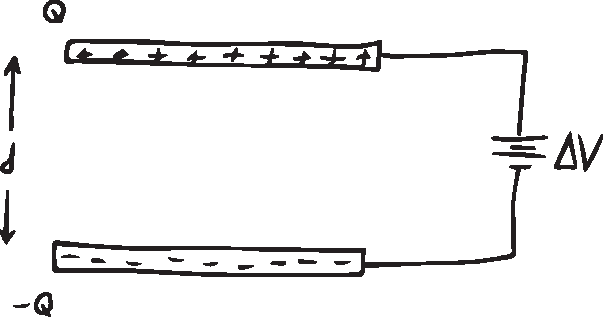
\includegraphics[scale=0.4]{../figures/condensateur-plan.pdf}
\end{center}

\begin{enumerate}
  \item Décrire le champ électrique entre les deux plaques.
  \item Déterminer le lien entre le champ électrique et la différence de
    potentiel.
  \item Montrer que la relation suivante est vraie
    $$Q = \frac{\epsilon_0 A}{d} \Delta V.$$
\end{enumerate}

\end{frame}


\begin{frame}[t]{Propriétés du condensateur plan}

Lesquels des énoncés suivants sont vrais.

\begin{enumerate}
  \item La charge accumulée sur un condensateur plan augmente
    proportionnellement à la différence de potentiel entre les plaques.
  \item Plus la distance entre les plaques est grande, plus la différence de
    potentiel doit être élevée pour maintenir la même charge sur les plaques.
  \item Si la densité surfacique de charge augmente et que la différence de
    potentiel demeure la même, la distance entre les plaques doit diminuer.
  \item Si on augmente la distance entre les plaques, l'énergie du système
    diminue.
  \item Si l'aire des plaques augmente, la capacité diminue.
  \item Plus la différence de potentiel entre les plaques augmente, plus la
    capacité diminue.
\end{enumerate}

\end{frame}


\begin{frame}[t]{Énergie dans un condensateur}

Considérons un condensateur avec une capacité $C$ dont les armatures sont
maintenues à une différence de potentiel $\Delta V$.

\begin{itemize}
  \item Si la charge sur la plaque est $q$, calculer l'énergie nécessaire pour
    amener une charge supplémentaire $dq$ sur la plaque.
  \item Déterminer l'énergie totale requise pour charger le condensateur avec
    une charge $Q$.
\end{itemize}

\end{frame}



\begin{frame}{Rigidité diélectrique}

\begin{center}
\begin{tabular}{lS}
  \toprule
  Substance       &        {Rigidité diélectrique (\si{V/cm})}     \\
  \midrule
  Air             &  30000  \\
  Verre           &  100000 \\
  Polystyrène     &  197000 \\
  Papier ciré     &  500000 \\
  Diamant         &  20000000 \\
  \bottomrule
\end{tabular}
\end{center}
\end{frame}



\begin{frame}{Exercice circuit avec condensateur}

On construit le circuit suivant avec une pile de \SI{9}{V}. Le condensateur 1 a
une capacité $C_1 = \SI{45}{\micro\farad}$ et ses armatures sont séparées par
du vide. Les condensateurs 2 et 3 sont construits exactement de la même façon que le
condensateur 1 sauf que tout l'espace entre leurs armatures est rempli par
du germanium et du papier, respectivement. La constante diélectrique du
germanium est 16 alors que celle du papier est 3.

\begin{center}
\begin{circuitikz}[scale=0.7]
  \draw (0, 0) to[battery, l=$\SI{9}{\volt}$] (0, 3)
    to[C, l=$C_1$] (2, 3)
    to[C, l=$C_2$] (2, 0)
    to (0, 0);
  \draw (2, 3) to[short] (4, 3)
    to[C, l=$C_3$] (4, 0)
    to (2, 0);
\end{circuitikz}
\end{center}

\begin{enumerate}
  \item Déterminer la capacité équivalente à ces trois condensateurs.
  \item Déterminer la charge accumulée sur la plaque positive du condensateur 2.
  \item Déterminer l'énergie accumulée dans le condensateur 3.
\end{enumerate}

\end{frame}

\end{document}
